\documentclass{article} % For LaTeX2e
\usepackage{nips15submit_e,times}
\usepackage{hyperref}
\usepackage{url}
\usepackage{lineno}
\usepackage{graphicx}
\graphicspath{ {images/} }
\usepackage{amsmath}
\usepackage[all]{hypcap} 
\usepackage{float}
%\linenumbers% Uncomment for line numbers



\title{Big Data, Big Problems--Parallelizing Kmeans}


\author{
Reuben K. McCreanor \\
Department of Statistics\\
Duke University\\
Durham, NC 27708 \\
\texttt{reuben.mccreanor@duke.edu} \\
\And
Wei (Emily) Shao\\
Department of Statistics\\
Duke University\\
Durham, NC 27708 \\
\texttt{wei.shao@duke.edu} \\
}

\hypersetup{
    colorlinks=true,
    linkcolor=blue,
    filecolor=magenta,      
    urlcolor=cyan,
    pdftitle={Sharelatex Example},
    bookmarks=true,
    pdfpagemode=FullScreen,
}


\newcommand{\fix}{\marginpar{FIX}}
\newcommand{\new}{\marginpar{NEW}}

\nipsfinalcopy 

\begin{document}

\maketitle

\begin{abstract}
K-means is a data-partitioning algorithm that separates n observations into k partitions. Due to its simplicity of implementation, its easy interpretability, and its ability to categorize data based on desired features, it remains one of the most popular algorithms in fields of statistics and machine learning. However, the key issue with k-means comes from its efficiency and scalability. As the size of datasets continues to increase, implementing k-means on data of any magnitude becomes computationally infeasible. A recently proposed variation of k-means, k-means++, provides a robust method of selecting the initial centers, essentially giving an optimal solution. However, due to the number of passes over the data required in a naive  implementation, even clusters a million data points into 100 partitions would be exceedingly slow. In order to combat this, a parallelized version of k-means++ is proposed, k-means $||$. This version uses a sampling factor $\ell$ to dramatically reduce the number of passes while still arriving at an equivalent solution of partitions. This paper will implement k-means++ and k-means$||$ in both sequential and parallel setting and compare the results both in terms of efficiency and equivalency of partition arrangements.
\end{abstract}

\section{Introduction}
\label{headings}

In general, clustering is a means of grouping observations into a set such that the other observations in this set are more similar to each other than to those in other sets. Starting with a data set, we use the use the k-means algorithm to define which observations are most similar to each other, and thus categorize these observations into k groups. 

\begin{figure}[H]
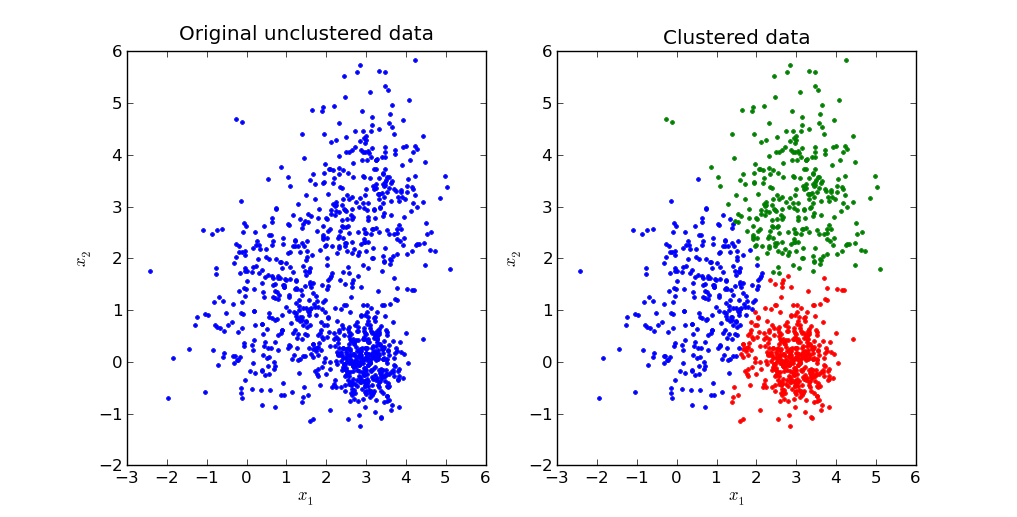
\includegraphics[width=10cm]{clusterEx}
\centering
\caption{The left hand side shows unclustered data, which the right hand side shows the same data categorized into three clusters}
\end{figure}

In the example above, we can data can be clustered into three partitions based on the similarity between observations. In industry, a common application of clusters is in market segmentation. Taking the example of Lenovo, an online hardware retailer, they use k-means clusters as a way of understand their total addressable market. Given that there total market is comprised of people from many different incomes, locations, and type of consumers, clustering allows them to understand which groups are most similar based on these attributes and thus design tarketing marketing campaigns for each discinct group. 



\section{Overview of the Algorithms}
\label{headings}

\subsection{K-means++}

\subsection{K-means$||$}

\section{Implementation}
\label{headings}

\subsection{Sudo Code}

\subsection{Data Simulation}

\subsection{Testing}

\section{Optimization}
\label{headings}

\subsection{Numba}

\subsection{Cython}

\subsection{MapReduce and Hadoop}

\section{Results}
\label{headings}

\subsection{Comparison of Numerical Results}

\subsection{Comparison Clustering Arrangements}

\subsection{Comparison of Efficiency}

\section{Conclusions}
\label{headings}

\clearpage
\newpage

\subsubsection*{References}

Bahmani, Bahman, Benjamin Moseley, Andrea Vattani, Ravi Kumar, and Sergei Vassilvitskii. \textit{Scalable K-means.} Proc. VLDB Endow. Proceedings of the VLDB Endowment 5.7 (2012): 622-33. Web.


\clearpage
\newpage

\section{Appendix}
\label{headings}



\end{document}


